\documentclass{article}

\usepackage[polish]{babel}
\usepackage{polski}
\usepackage[utf8]{inputenc}
\usepackage{longtable}
\usepackage{array}
\usepackage{enumitem}
\usepackage{makecell}
\usepackage{amsmath}
\usepackage{longtable}
\usepackage{graphicx}
\usepackage{float}
\usepackage{listings}
\usepackage[colorlinks=true, linkcolor=black]{hyperref}
\usepackage[letterpaper,top=2cm,bottom=2cm,left=3cm,right=3cm,marginparwidth=1.75cm]{geometry}

\renewcommand{\familydefault}{\sfdefault}

\title{Zastosowanie algorytmu mrówkowego do rozwiązania problemu Capacitated Vehicle Routing Problem \\ \large{Raport końcowy}}
\author{Jan Szablanowski}

\begin{document}
\date{}
\maketitle

\vspace{2cm}
% \newpage
\hypersetup{
    linkcolor=black,
    citecolor=black,
    urlcolor=black
}

\abstract{}

Repozytorium kodu zostało umieszczone na GitHub: \url{https://github.com/r-ost/MSI2-ants}

\tableofcontents
\newpage


% opis problemu (uzupełniony z konspektu),
% sprawdzone hipotezy i opis eksperymentów, które posłużyły do ich weryfikacji (rozszerzona wersja z konspektu)
% wyniki eksperymentów przedstawione w sposób przystępny dla czytelnika – nie w formie surowych tabel z pojedynczymi wartościami,
% wniosków, w tym stwierdzenia czy postawione hipotezy są prawdziwe,
% raport powinien zawierać odnośniki bibliograficzne do literatury, publikacji recenzowanych,
% streszczenie na około 250 słów podsumowujące eksperymenty i najważniejsze wyniki.

\section{Opis problemu}

Capacitated Vehicle Routing Problem (CVRP) to problem optymalizacyjny, który jest rozszerzeniem problemu marszrutyzacji (Vehicle Routing Problem - VRP). W zadaniu VRP mamy dany nieskierowany graf pełny oraz ustaloną liczbę pojazdów. Wierzchołki grafu, poza jednym, oznaczają lokalizacje klientów na płaszczyźnie. Jeden wierzchołek jest wyszczególniony i oznacza magazyn. Krawędzie w grafie mają przypisane wagi, które oznaczają odległości między wierzchołkami. Celem problemu VRP jest odwiedzenie każdego klienta dokładnie raz, minimalizując całkowity koszt przebycia tras wszystkich pojazdów. Każda trasa zaczyna się i kończy w magazynie. W CVRP dodatkowo każdy klient ma określone zapotrzebowanie na jeden, określony produkt, a każdy pojazd może przewozić skończoną ilość produktu. W ramach projektu zakładamy dodatkowo, że droga, którą może przebyć każdy z pojazdów, jest ograniczona przez pewną stałą.
\\ \\
Problem CVRP jest NP-trudny \cite{lenstra}. W związku z tym dokładne rozwiązanie można wyznaczyć tylko dla małych instancji (rzędu kilku-kilkunastu wierzchołków). W praktyce problem CVRP rozwiązuje się, znajdując przybliżone rozwiązanie. W projekcie zostaną porównane cztery algorytmy znajdujące przybliżone rozwiązanie problemu CVRP:
\begin{enumerate}
    \item Algorytm mrówkowy
    \item Algorytm mrówkowy z heurystyką 2-opt
    \item Algorytm mrówkowy z modyfikacją Max-Min (Max-Min ant system - MMAS)
    \item Algorytm zachłanny
\end{enumerate}

\section{Opis algorytmów}
\subsection{Algorytm zachłanny}
Algorytm zachłanny jest prostą heurystyką, którą można zastosować do problemu CVRP. Algorytm ten podejmuje decyzje lokalnie optymalne, licząc na uzyskanie globalnie optymalnego rozwiązania. W  przypadku problemu CVRP, w każdym kroku algorytm wybiera najbliższego klienta, który jednocześnie spełnia ograniczenia pojemności pojazdu i limitu długości trasy. Procedura powtarzana jest dla kolejnych pojazdów, aż do obsłużenia wszystkich klientów.
\\ \\
Algorytm zachłanny podejmuje decyzje lokalnie bez uwzględnienia przyszłych konsekwencji swoich decyzji, co może prowadzić do rozwiązań słabej jakości względem algorytmu mrówkowego. Niewątpliwą zaletą algorytmu zachłannego jest za to łatwość implementacji i szybkość działania, co może mieć znaczenie przy złożonych problemach i dużych danych wejściowych.

\subsection{Algorytm mrówkowy}
Algorytm mrówkowy (Anto Colony Optimization - ACO) \cite{dorigo} to meta-heurystyczne podejście do rozwiązywania problemów trudnych obliczeniowo, które jest inspirowane zachowaniem kolonii mrówek. Mrówki podczas przemieszczania się pozostawiają po sobie ślady w postaci feromonów, którymi podążają inne mrówki. Z biegiem czasu najmocniejsze ślady powstają na najkrótszych ścieżkach, ponieważ mrówki mogą się nimi przemieszczać najszybciej.
\\ \\
Algorytm mrówkowy działa w iteracjach. Każda iteracja zawiera następujące kroki:
\subsubsection*{1. Wygenerowanie pełnego rozwiązania przez każdą mrówkę na podstawie probabilistycznej funkcji przejścia}
\begin{equation}
    P_{ij} = \frac{(\tau_{ij})^\alpha \cdot (\eta_{ij})^\beta}{\sum_{k \in N_i} (\tau_{ik})^\alpha \cdot (\eta_{ik})^\beta}
\end{equation}
gdzie:
\\
$P_{ij}$ - prawdopodobieństwo przejścia z wierzchołka $i$ do wierzchołka $j$,
\\
$\tau_{ij}$ - ilość feromonu na krawędzi $i$-$j$,
\\
$\eta_{ij}$ - heurystyka (odwrotność odległości między wierzchołkami $i$ i $j$),
\\
$\alpha$ - waga feromonu,
\\
$\beta$ - waga heurystyki,
\\
$N_i$ - zbiór wierzchołków, do których mrówka może przejść z wierzchołka $i$.

\subsubsection*{2. Obliczenie jakości rozwiązania i zaktualizowania najlepszego dotychczasowego rozwiązania.}

\subsubsection*{3. Zaktualizowanie śladów feromonowych, uwzględniając osłabianie się feromonów.}

\begin{equation}
    \tau_{ij} = (1 - \rho) \cdot \tau_{ij} + \sum_{k=1}^{m} \Delta\tau_{ij}^k
\end{equation}
gdzie:
\\
$\rho$ - współczynnik parowania feromonu, 
\\
$m$ - liczba mrówek, 
\\
$\Delta\tau_{ij}^k$ - ilość feromonu dodanego przez mrówkę $k$ na krawędzi $i$-$j$.
\\ \\
Ilość feromonu dodanego przez mrówkę $k$ na krawędzi $i$-$j$ jest obliczana na podstawie jakości rozwiązania, które mrówka znalazła. Im lepsze rozwiązanie, tym więcej feromonu zostaje dodane do krawędzi.

\begin{equation}
    \Delta\tau_{ij}^k = \frac{Q}{L_k}
\end{equation}
gdzie:
\\
$Q$ - stała,
\\
$L_k$ - długość trasy mrówki $k$.


\subsection{Algorytm mrówkowy z heurystyką 2-opt}
Heurystyka 2-opt jest lokalną heurystyką, która polega na poprawie jakości rozwiązania poprzez wybór dwóch wierzchołków na trasie o indeksach $i$, $j$ i usunięcie krawędzi $i - 1$-$i$ oraz $j$-$j+1$. Następnie krawędzie między wierzchołkami $i$ i $j$ są dodawane w odwrotnej kolejności. Na koniec dodawane są krawędzie $i-1$-$j$ oraz $i$-$j+1$.
\\ \\
Heurystyka 2-opt pozwala na usunięcie przecięcia tras, co prowadzi do skrócenia całkowitej długości trasy. Heurystyka ta jest stosowana po wygenerowaniu trasy przez algorytm mrówkowy. Algorytm mrówkowy z heurystyką 2-opt działa w następujący sposób \cite{tan}:
\begin{enumerate}
    \item Algorytm mrówkowy generuje trasę dla każdego pojazdu.
    \item Dla każdej trasy algorytm mrówkowy stosuje heurystykę 2-opt, aby poprawić jakość rozwiązania.
    \item Algorytm aktualizuje feromony na krawędziach zgodnie z jakością rozwiązania.
\end{enumerate}
Heurystyka 2-opt jest stosunkowo prosta do zaimplementowania i może znacznie poprawić jakość rozwiązań. W przypadku problemu CVRP, heurystyka 2-opt może być szczególnie skuteczna, ponieważ pozwala na poprawę jakości tras, które są już bliskie optymalnym.

\subsection{Algorytm mrówkowy z modyfikacją Max-Min}

Algorytm mrówkowy z modyfikacją Max-Min (Max-Min Ant System - MMAS) \cite{maxmin} to rozwinięcie klasycznego algorytmu mrówkowego, które wprowadza zmiany w sposobie aktualizacji feromonu. W MMAS feromon na krawędzi jest aktualizowany tylko przez najlepszą mrówkę w danej iteracji lub globalnie. Zwiększa to koncentrację feromonu na najlepszych krawędziach, co prowadzi do szybszej konwergencji algorytmu i większej eksploatacji. Dodatkowo, w MMAS wprowadza się ograniczenia na minimalną i maksymalną ilość feromonu na krawędziach oraz maksymalną liczbę iteracji bez poprawy, po której algorytm resetuje feromony. Dzięki temu algorytm jest bardziej stabilny i mniej podatny na stagnację. 


\section{Sprawdzone hipotezy}
W projekcie postawiono cztery hipotezy, których celem było porównanie jakości rozwiązań uzyskiwanych przez różne algorytmy. Hipotezy były testowane na zbiorze Uchoa et al. (2014) \cite{Uchoa} z bazy CVRLIB (Capacitated Vehicle Routing Problem Library), która zawiera 100 różnorodnych instancji problemu, w których występuje od 100 do 1000 klientów. W testowaniu hipotez wykorzystano 6 instancji problemu CVRP o różnych rozmiarach i rozkładach klientów. Przykładowa instancja została pokazana na rysunku \ref{fig:n101}, a jej rozwiązanie na rysunku \ref{fig:n214}. 
\\ \\
Algorytmy mrówkowe wraz z modyfikacjami 2-opt i Max-Min były uruchamiane 3 razy na każdej instancji z różnymi ziarnami (wyniki były potem uśredniane). Parametry algorytmu mrówkowego i liczba iteracji były takie same dla wszystkich instancji z wyjątkiem algorytmu mrówkowego z modyfikacją Max-Min, w którym początkową liczbę feromonów ustawiono jako maksymalną liczbę feromonu. Wartości parametrów algorytmu mrówkowego były ustalane na podstawie literatury i własnych eksperymentów i przedstawiono je w tabeli \ref{tab:params}.

% TODO dwie przykladowe instancje problemu
\begin{figure}[H]
    \centering
    \begin{minipage}{0.48\textwidth}
        \centering
        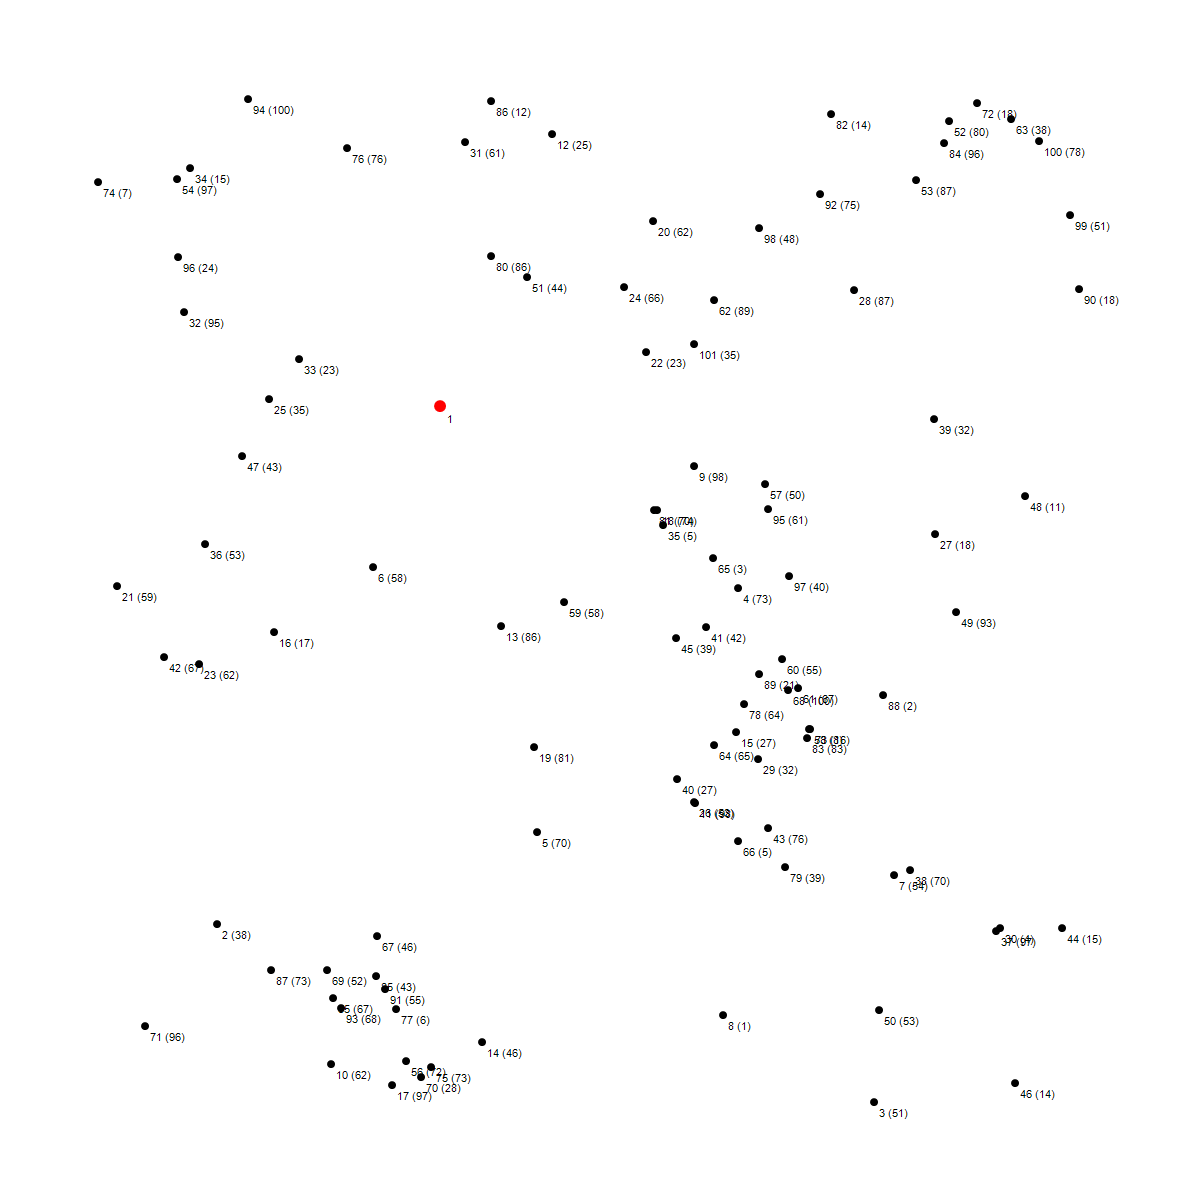
\includegraphics[width=\linewidth]{img/20250405_224145_X-n101-k25.png}
        \caption{Instancja \texttt{X-n101-k25} -- wierzchołki oznaczono jako: \texttt{IdKlienta(Zapotrzebowanie)}. Magazyn oznaczono na czerwono}
        \label{fig:n101}
    \end{minipage}
    \hfill
    \begin{minipage}{0.48\textwidth}
        \centering
        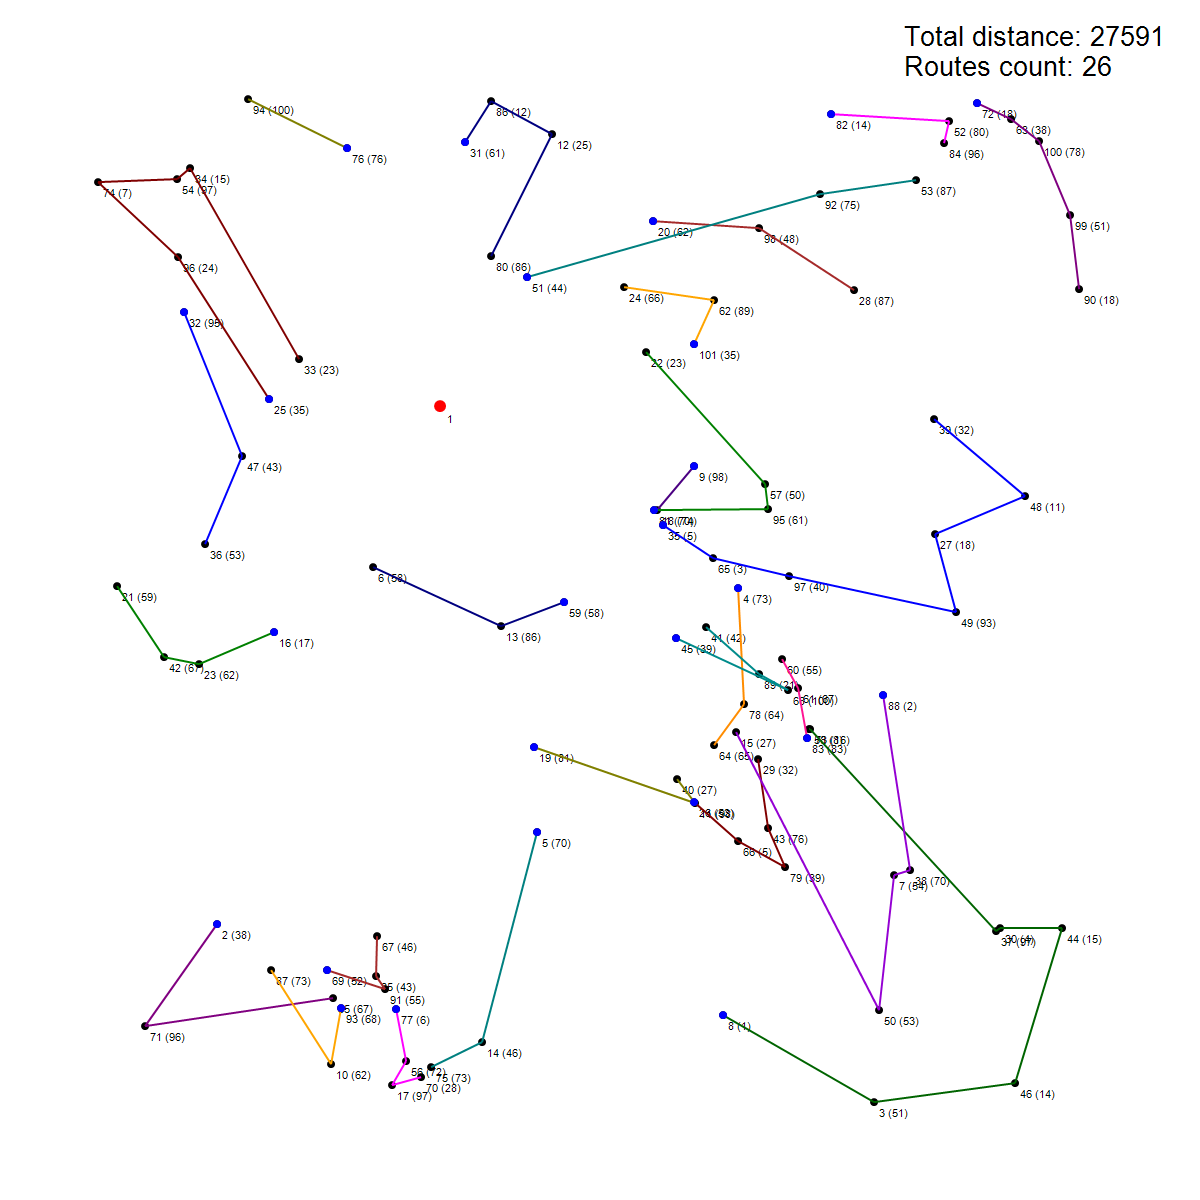
\includegraphics[width=\linewidth]{img/20250407_002013_X-n101-k25_optimal.png}
        \caption{Optymalne rozwiązanie instancji \texttt{X-n101-k25}}
        \label{fig:n214}
    \end{minipage}
\end{figure}

% TODO: tabela z parametrami algorytmu mrówkowego i modyfikacji Max-Min
% MaxIterations = 100,
% Alpha = 1.0,
% Beta = 5.0,
% EvaporationRate = 0.2,
% Q = 10,
% InitialPheromone = 0.1,
\begin{table}[H]
    \label{tab:params}
    \centering
    \begin{tabular}{|c|c|c|c|c|}
        \hline
        \textbf{Parametr} & \textbf{Wartość} \\
        \hline
        Liczba mrówek & Równa liczbie wierzchołków w grafie \\
        \hline
        Liczba iteracji & 100 \\
        \hline
        Współczynnik parowania feromonu ($\rho$) & 0.2 \\
        \hline
        Waga feromonu ($\alpha$) & 1 \\
        \hline
        Waga heurystyki ($\beta$) & 5 \\
        \hline
        Ilość dodawanego feromonu ($Q$) & 10 \\
        \hline
        Początkowa ilość feromonu & 0.1 \\
        \hline
    \end{tabular}
    \caption{Parametry algorytmu mrówkowego}
    \label{tab:params}
\end{table}

\subsection{Hipoteza 1}
\textit{Algorytm mrówkowy z heurystyką 2-opt znajduje trasy o co najmniej 10\% mniejszym koszcie w porównaniu do klasycznego algorytmu mrówkowego.}
\\
\textbf{Wynik: Częściowo prawdziwa dla dużych instancji.} 
\\ \\
Celem tego eksperymentu było sprawdzenie, czy heurystyka 2-opt rzeczywiście poprawia jakość rozwiązań uzyskiwanych przez algorytm mrówkowy. W tym celu porównano wyniki uzyskane przez algorytm mrówkowy z heurystyką 2-opt z wynikami uzyskanymi przez klasyczny algorytm mrówkowy.


\begin{figure}[H]
    \centering
    \begin{minipage}{0.48\textwidth}
        \centering
        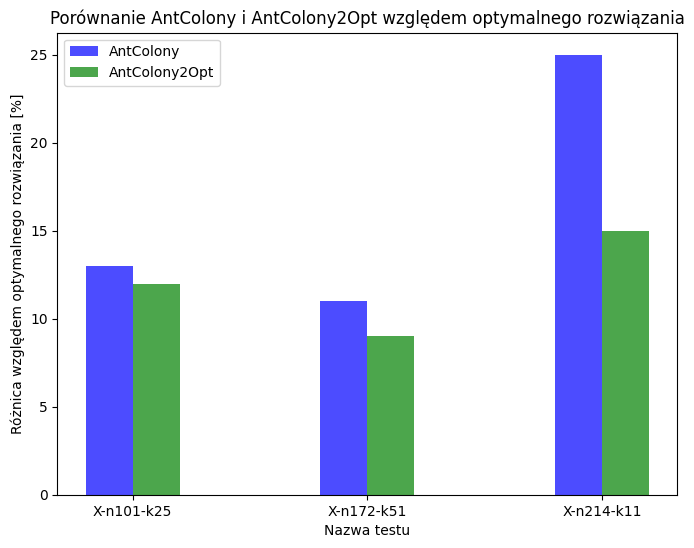
\includegraphics[width=\linewidth]{img/2opt_wzgledem_optymalnego.png}
        \caption{Długość rozwiązania ACO i ACO 2-opt względem optymalnego}
        \label{fig:2opt_wzgledem_optymalnego}
    \end{minipage}
    \hfill
    \begin{minipage}{0.48\textwidth}
        \centering
        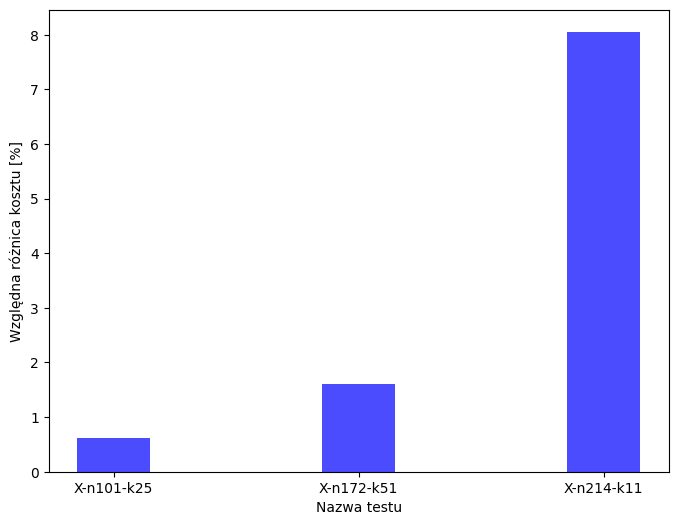
\includegraphics[width=\linewidth]{img/2opt_wzgledem_zwyklego.png}
        \label{fig:2opt_wzgledem_zwyklego}
        \caption{O ile procent AntColony2Opt jest lepszy od AntColony?}
    \end{minipage}
\end{figure}
\noindent Z rysunku \ref{fig:2opt_wzgledem_optymalnego} widać, że dla wszystkich instancji testowych algorytm mrówkowy z heurystyką 2-opt znalazł rozwiązania o niższym koszcie niż klasyczny algorytm mrówkowy. Rysunek \ref{fig:2opt_wzgledem_zwyklego} pokazuje, że względna różnica w długościach rozwiązań jest mniejsza niż 10\%. W przypadku instancji o największej liczbie klientów (214) różnica ta wynosi około 8\%, natomiast w przypadku instancji o najmniejszej liczbie klientów (101) różnica ta wynosi mniej niż 1\%. Widać z tego, że różnica w długości rozwiązań rośnie wraz ze wzrostem liczby wierzchołków i hipoteza ma szansę być prawdziwa dla dużych instancji problemu CVRP.

\subsection{Hipoteza 2}
\textit{Algorytm mrówkowy z modyfikacją Max-Min znajduje rozwiązanie o koszcie nie większym niż 5\% od kosztu rozwiązania znalezionego przez klasyczny algorytm mrówkowy, ale potrzebuje do tego o 10\% mniejszej liczby pojazdów.}
\\
\textbf{Wynik: Fałszywa.}
\\ \\
\noindent Celem tego eksperymentu było sprawdzenie, czy algorytm mrówkowy z modyfikacją Max-Min znajduje rozwiązania o większej jakości niż klasyczny algorytm mrówkowy. Jakość rozwiązania jest tutaj rozumiana jako poziom wykorzystania pojemności pojazdów i wiąże się z mniejszą liczbą pojazdów potrzebnych do obsłużenia wszystkich klientów. Użyte wartości parametrów związanych z modyfikacją Max-Min przedstawiono w tabeli \ref{tab:maxmin_params}.

\begin{table}[H]
    \centering
    \begin{tabular}{|c|c|c|c|}
        \hline
        \textbf{Parametr} & \textbf{Wartość} \\
        \hline
        Minimalna ilość feromonu & 0.01 \\
        \hline
        Maksymalna ilość feromonu & 10 \\
        \hline
        Początkowa ilość feromonu & 10 \\
        \hline
        Maksymalna liczba iteracji bez poprawy & 20 \\
        \hline
    \end{tabular}
    \caption{Dodatkowe parametry algorytmu Max-Min}
    \label{tab:maxmin_params}
\end{table}

\begin{figure}[H]
    \centering
    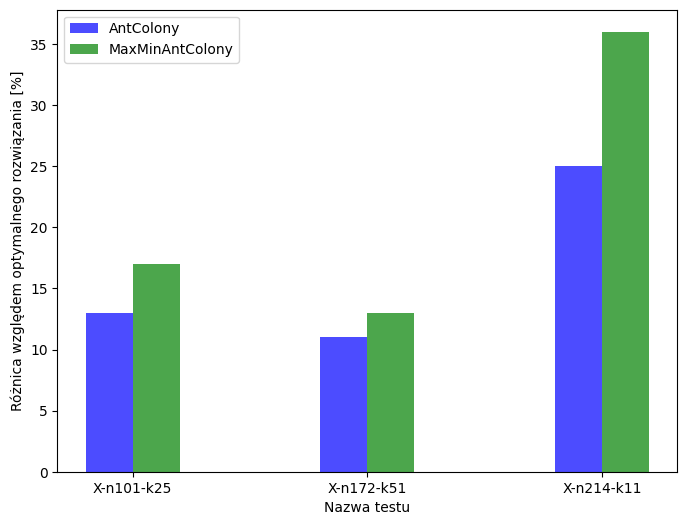
\includegraphics[width=0.48\linewidth]{img/maxmin_wzgledem_optymalnego.png}
    \caption{Długość rozwiązania ACO i MMAS względem optymalnego}
    \label{fig:MMAS_wzgledem_optymalnego}
\end{figure}

\begin{figure}[H]
    \centering
    \begin{minipage}{0.48\textwidth}
        \centering
        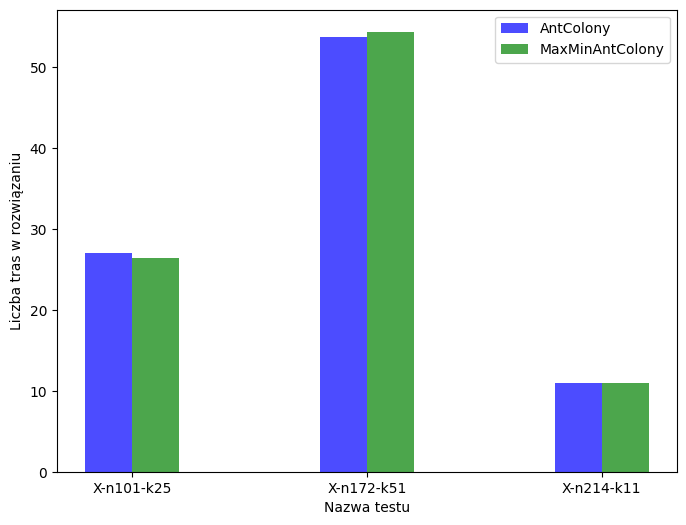
\includegraphics[width=\linewidth]{img/maxmin_trasy.png}
        \caption{Liczba tras dla ACO i MMAS}
        \label{fig:maxmin_trasy}
    \end{minipage}%
    \hfill
    \begin{minipage}{0.48\textwidth}
        \centering
        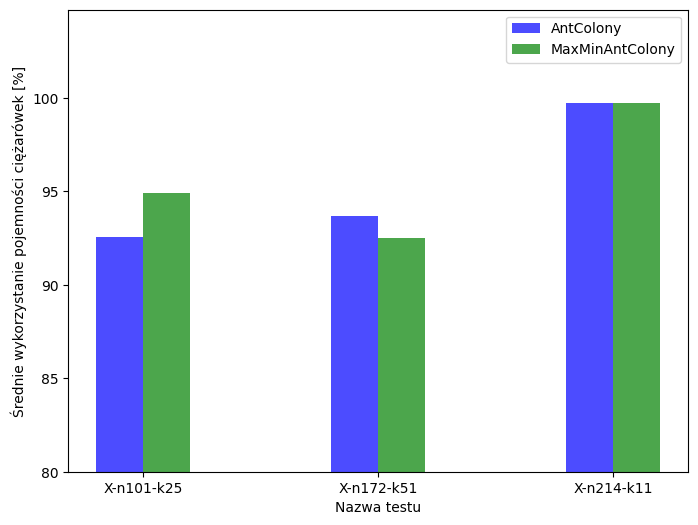
\includegraphics[width=\linewidth]{img/max_min_capacity.png}
        \caption{Średnie wykorzystanie pojemności pojazdów na trasach}
        \label{fig:max_min_capacity}
    \end{minipage}
\end{figure}

\noindent Na rysunku \ref{fig:MMAS_wzgledem_optymalnego} widać, że algorytm mrówkowy z modyfikacją Max-Min znajduje rozwiązania o większym koszcie niż klasyczny algorytm mrówkowy. Różnica ta jest rzędu kilku-kilkunastu procent, co było spodziewane przy formułowaniu hipotezy. Z rysunku \ref{fig:maxmin_trasy} widać jednak, że algorytm mrówkowy z modyfikacją Max-Min potrzebuje porównywalnej liczby tras jak klasyczny algorytm mrówkowy i zależy to od problemu. Podobnie jest ze średnim wykorzystaniem pojemności pojazdów na trasach, które jest porównywalne dla obu algorytmów (rysunek \ref{fig:max_min_capacity}). Wynik eksperymentu, który obala hipotezę, może wynikać z nieprawidłowego doboru parametrów albo zbyt małej liczby iteracji w testach algorytmu mrówkowego z modyfikacją Max-Min.

\subsection{Hipoteza 3}
\textit{Procentowa różnica kosztów wyznaczonych tras między algorytmem zachłannym i klasycznym algorytmem mrówkowym rośnie wraz ze wzrostem liczby klientów na niekorzyść algorytmu zachłannego.}
\\
\textbf{Wynik: Potwierdzona hipoteza przeciwna.}
\\ \\
Celem eksperymentu było sprawdzenie, czy różnica w kosztach wyznaczonych tras między algorytmem zachłannym i klasycznym algorytmem mrówkowym rośnie wraz ze wzrostem liczby klientów. Hipoteza wynikała z przypuszczenia, że algorytm zachłanny nie jest w stanie znaleźć dobrego rozwiązania dla dużych instancji problemu CVRP, ponieważ podejmuje decyzje lokalnie optymalne.

\begin{figure}[H]
    \centering
    \begin{minipage}{0.48\textwidth}
        \centering
        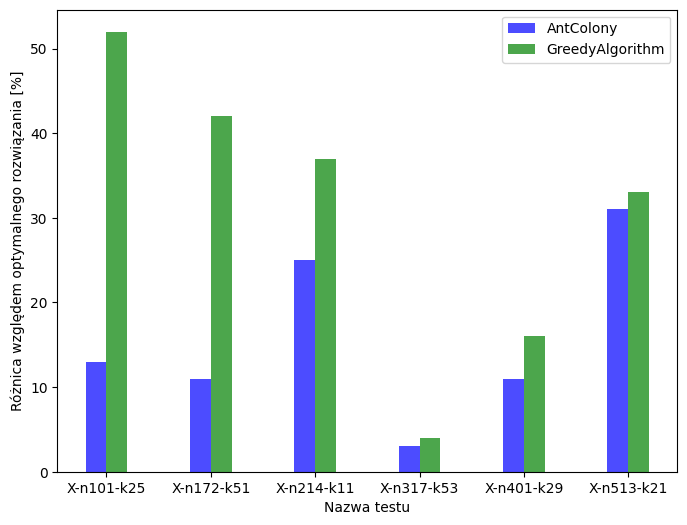
\includegraphics[width=\linewidth]{img/greed_wzgledem_optymalnego.png}
        \caption{Długość rozwiązania ACO i Greedy względem optymalnego}
        \label{fig:greedy_wzgledem_optymalnego}
    \end{minipage}
    \hfill
    \begin{minipage}{0.48\textwidth}
        \centering
        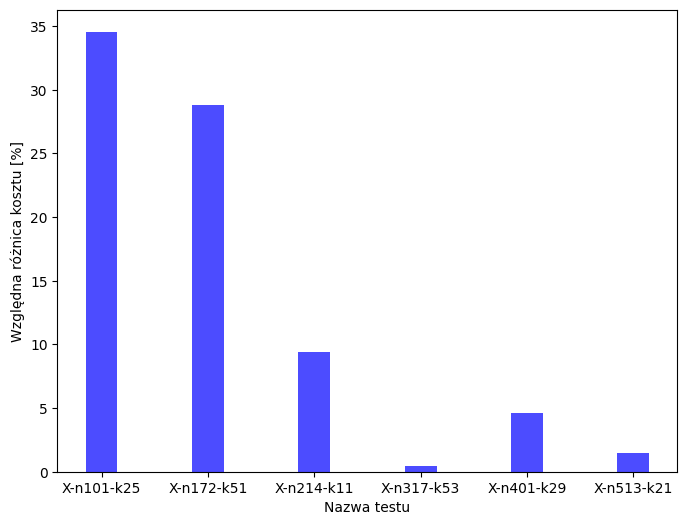
\includegraphics[width=\linewidth]{img/greedy_wzgledem_zwyklego.png}
        \caption{O ile procent ACO jest lepszy od Greedy?}
        \label{fig:greedy_wzgledem_zwyklego}
    \end{minipage}
\end{figure}
\noindent Na rysunku \ref{fig:greedy_wzgledem_optymalnego} widać, że algorytm ACO znajduje rozwiązania o mniejszym koszcie niż algorytm zachłanny dla każdej instancji testowej, co było spodziewane.
Jednakże na rysunku \ref{fig:greedy_wzgledem_zwyklego} widać, że różnica w długości rozwiązań maleje wraz ze wzrostem liczby klientów na korzyść algorytmu zachłannego, co potwierdza hipotezę odwrotną do postawionej (liczba klientów ujęta jest w nazwie instancji po literze \texttt{n}).

\subsection{Hipoteza 4}
\textit{Procentowa różnica kosztów wyznaczonych tras między algorytmem mrówkowym z heurystyką 2-opt i klasycznym algorytmem mrówkowym rośnie wraz ze wzrostem rozproszenia klientów (mierzonego średnią odległością klientów od magazynu) na niekorzyść klasycznego algorytmu.}

\section{Wnioski}


\nocite{*}
\bibliographystyle{unsrt}
\bibliography{../ref.bib}

\end{document}